\documentclass[11pt]{standalone}
\usepackage[usenames]{color} %used for font color
\usepackage{amssymb} %maths
\usepackage{amsmath} %maths

\usepackage[no-math]{fontspec}
\usepackage{unicode-math}
\usepackage{libertinus}

\usepackage{pgf,xcolor}
\definecolor{itwm_blue_04}{HTML}{005A94}
\definecolor{itwm_red}{HTML}{C00000}
\definecolor{itwm_yellow}{HTML}{FFEC7F}

\usepackage{tikz}
\usetikzlibrary{shapes.misc, shadows, decorations, arrows}
\usetikzlibrary{backgrounds}
\usetikzlibrary{calc}
\usepackage{pgfplots}
\pgfplotsset{compat=newest}
\usepgfplotslibrary{fillbetween}
\usepackage{tikzpagenodes}

\begin{document}
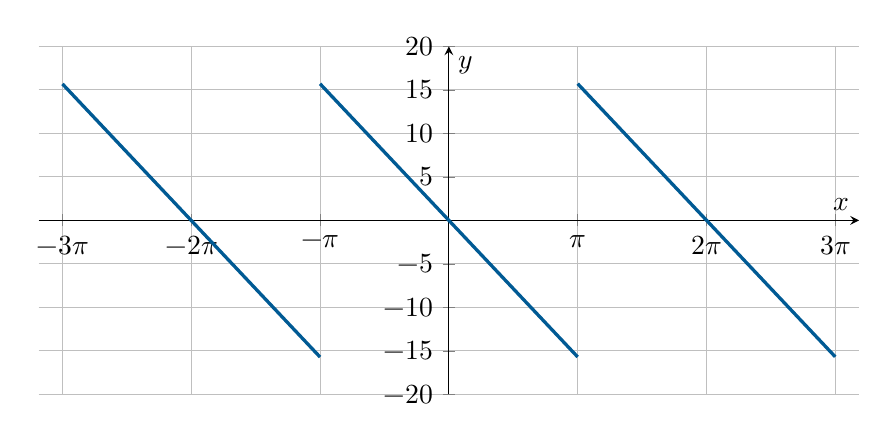
\begin{tikzpicture}
\begin{axis}[
    domain=-10:10,
    axis lines = center,
    xlabel = {$x$},
    ylabel = {$y$},
    height=6cm, width=12cm, 
    xmin=-10, xmax=10, ymin=-20, ymax=20, 
    ytick={-20,-15,...,20},
    xtick={-9.42,-6.28,...,9.42},
    xticklabels={$-3\pi$,$-2\pi$, $-\pi$, $0$, $\pi$, $2\pi$, $3\pi$},
    grid = both
]
\path [name path=xaxis]
      (\pgfkeysvalueof{/pgfplots/xmin},0) --
      (\pgfkeysvalueof{/pgfplots/xmax},0);
\addplot[draw=itwm_blue_04, smooth, very thick, name path=f, domain=-9.42:-3.14]{-5*(x+2*pi)};
\addplot[draw=itwm_blue_04, smooth, very thick, name path=f, domain=-3.14:3.14]{-5*x};
\addplot[draw=itwm_blue_04, smooth, very thick, name path=f, domain=3.14:9.42]{-5*(x-2*pi)};
\end{axis}
\end{tikzpicture}\end{document}